\documentclass[handout]{ximera}

\title{Learning Ximera, part 2!}
\author{Hilary Freeman}



\begin{document}
\begin{abstract}
  This is my second place to get started.
\end{abstract}
\maketitle

I will put some more problems here and ask for answers.

\begin{image}
  \begin{tikzpicture}
    \begin{axis}[
        width=6in,
        height=3in,
        xmin=-.5, xmax=5.5,ymin=-1.2,ymax=1.2,domain=0:6,
        axis lines =center, xlabel=$x$, ylabel=$y$,
        every axis y label/.style={at=(current axis.above origin),anchor=south},
        every axis x label/.style={at=(current axis.right of origin),anchor=west},
        axis on top,
    ] 
      \addplot [draw=none, %pattern=north west lines, pattern color=blue, fill=fillp,
        domain=0:1] {x} \closedcycle;
      \addplot [draw=none, %pattern=north west lines, pattern color=blue, fill=fillp,
        domain=1:5] {1.5-x/2} \closedcycle;

  \end{axis}
  \end{tikzpicture}
\end{image}

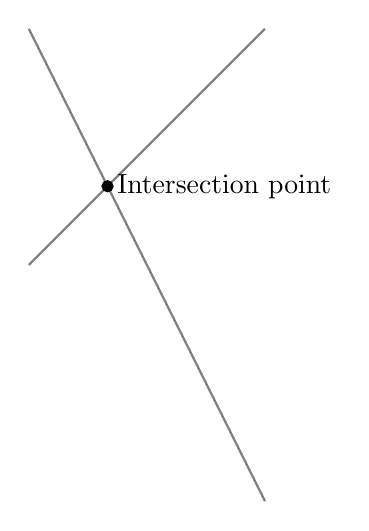
\begin{tikzpicture}
\draw[gray, thick] (-1,2) -- (2,-4);
\draw[gray, thick] (-1,-1) -- (2,2);
\filldraw[black] (0,0) circle (2pt) node[anchor=west] {Intersection point};
 
\end{tikzpicture}

\end{document}
